%%A Presentation by Krishna Vaidyanathan

\documentclass[aspectratio=169]{beamer}

\usepackage{hyperref}
\usepackage{color}
\usepackage{multirow}
%\usepackage[font=tiny,labelfont=bf]{caption}[numbered]

%% Smart underlining -- from cdi-macros.tex
\def\ul#1{$\underline{\smash{\hbox{#1}}}$}

%% Shortcuts

\newcommand{\tabitem}{~~\llap{\textbullet}~~}

\newcommand{\bd}{\begin{description}}
\newcommand{\ed}{\end{description}}

\mode<presentation>
{
  \usetheme{Madrid}
  \useinnertheme{circles}
  \usecolortheme{beaver}
}
\usepackage[english]{babel}

\usepackage{times}
\usepackage[T1]{fontenc}
%
\title[IceFS]{Physical Disentanglement in a Container-Based File System}
\subtitle{A Presentation for CS854}
\author[Presented by Krishna Vaidyanathan]{Lanyeu Lue,\\Yupu Zhang,\\Thanh
    Do,\\Samer Al-Kiswany,\\Andrea C. Arpaci-Dussueau,\\Remzi
    H. Arpaci-Dussueau\\\vspace{2em}Presented by Krishna Vaidyanathan}

\date{March 4, 2016}
\newcommand{\bi}{\begin{itemize}}
\newcommand{\ei}{\end{itemize}}

\newcommand{\bn}{\begin{enumerate}}
\newcommand{\en}{\end{enumerate}}

\begin{document}

\frame[plain]{\titlepage}

\begin{frame}{Table of Contents}
\tableofcontents
\end{frame}

\section{Introduction}
\begin{frame}{Introduction}
    \bi
\item Isolation is central to increased reliability and improved performance of
    modern computer systems.
\item We say, for example, that two files are \textit{entangled} if their
    blocks are allocated using the same bitmap.
\item Entanglement mainly arises because:
    \bi
\item Logically-independent file system entities are not physically independent.
    \ei
    \ei
\end{frame}

\section{Motivation}
\begin{frame}{Motivation}
    \bi
\item Entanglement can cause three main problems:
    \bn
\item Global failure
\item Slow recovery
\item Bundled performance
    \en
    \ei
\end{frame}

\begin{frame}{Motivation: Global Failure}
    \begin{columns}[T]
        \begin{column}{0.5\textwidth}
        \bi
    \item Single fault leads to a global failure.
    \item Current file systems crash entire system or mark whole file system read
        -only.
    \item For example:
        \bi
    \item Btrfs crashes entire OS when invariant is violated.
    \item ext3 marks whole file-system read-only when it detects corruption in
        single inode bitmap.
        \ei
        \ei
\end{column}
\hspace{-2cm}\begin{column}{0.2\textwidth}
    \pause
    \begin{figure}\flushleft
        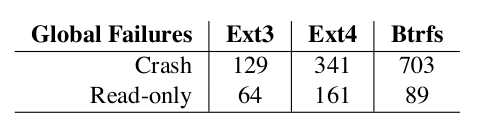
\includegraphics[scale=0.3]{./figures/table1.png}
    \end{figure}
    \pause
    \begin{figure}\flushleft
        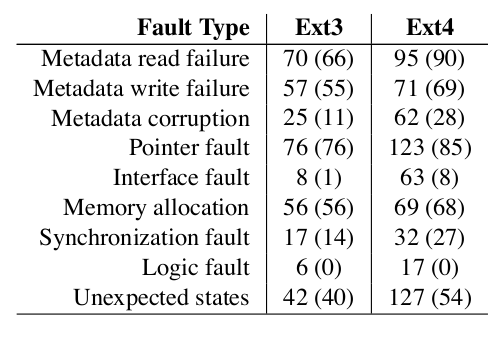
\includegraphics[scale=0.3]{./figures/table2.png}
    \end{figure}
\end{column}
\end{columns}
\end{frame}

\begin{frame}{Motivation: Slow Recovery}
    \begin{columns}[T]
        \begin{column}{0.4\textwidth}
        \bi
    \item After failure, offline file-system checker scans whole file system.
    \item Checkers are pessimistic: entire file system checked, when only a small
        piece of corrupted data.
    \item Not scalable.
        \ei
    \end{column}
    \begin{column}{0.2\textwidth}
        \pause
        \begin{figure}
            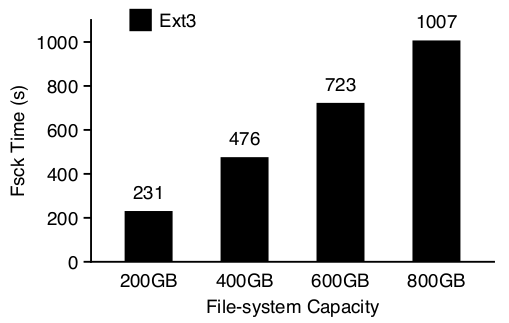
\includegraphics[scale=0.3]{./figures/fig1.png}
        \end{figure}
    \end{column}
    \end{columns}
\end{frame}

\begin{frame}{Motivation: Bundled Performance}
    \begin{columns}[T]
        \begin{column}{0.4\textwidth}
            \bi
        \item File-systems, like ext3, use a journal to keep track of uncommitted changes,
            committing at periodic intervals.
        \item All updates within a short period of time are grouped together.
        \item Performance of independent processes are bundled.
            \ei
    \end{column}
    \begin{column}{0.2\textwidth}
        \pause
        \begin{figure}
            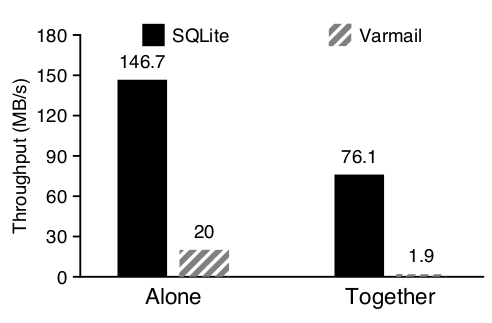
\includegraphics[scale=0.3]{./figures/fig2.png}
        \end{figure}
    \end{column}
\end{columns}
\end{frame}

\section{Current Solutions}
\begin{frame}{Current Solutions}
    \bi
\item Namespaces: defines subset of files and directories to be made visible.
    \pause
    \bi
\item Fails to address above problems.
\item Files from different namespaces may still share metadata, system states
    etc.,
    \ei
\item Static disk partitions: Multiple file systems can be created on separate
    partitions.
    \pause
    \bi
\item Single \texttt{panic()} or \texttt{BUG\_ON()} can still crash entire OS.
\item Not flexible, and number of partitions limited.
    \ei
    \ei
\end{frame}

\section{Usage Scenarios}
\begin{frame}{Usage Scenarios}
    \bi
\item Virtual Machines:
    \bi
    \pause
\item Fault isolation of paramount importance.
\item Single fault triggered by one virtual disk can cause host file system to
    become read-only.
\item Redeployment and recovery require considerable downtime.
    \ei
    \pause
\item Distributed File Systems:
    \bi
    \pause
\item Physical entanglement negatively impacts distributed file systems, especially multi-tenant
    settings.
\item Specifically, HDFS does not provide fault isolation for applications.
\item Eg: four clients concurrently read different files, and the machine
    which stores the data blocks crashes.
    \ei
    \ei
\end{frame}

\begin{frame}{Cube Abstraction}
    \bi
\item Enables logical relation between files and directories.
\item Safely combine performance and reliability properties of groups of files
    and their metadata.
\item Each cube is completely independent at the file-system level.
\item Cubes are:
    \bn
\item Isolated
\item Transparent
\item Flexible
\item Elastic
\item Customized
\item Lightweight
    \en
    \ei
\end{frame}

\section{Principles of Disentangled Data Structures}
\begin{frame}{Principles: No Shared Physical Resources}
    \bi
\item Storage space is divided into fixed-size block groups.
\item Each block group has its own metadata.
\item Files and directories are allocated to particular block groups.
\item Any block group and its corresponding metadata blocks can be shared across
    any set of files.
    \ei
\end{frame}

\begin{frame}{Principles: No Access Dependency}
    \bi
\item Cubes must not contain references/need access to other cubes.
\item Data structures that violate this: linked list, trees etc.,
\item One failed entry can affect all entries above or below it.
    \ei
\end{frame}

\begin{frame}{Principles: No Bundled Transactions}
    \bi
\item To guarantee consistency and metadata, existing file-systems use
    journaling.
\item A transaction for this contains temporal updates from many files.
\item Problems:
    \bi
\item Updates to all files in transition fails.
\item Performance of independent files and workloads coupled.
    \ei
    \ei
\end{frame}

\section{IceFS}
\begin{frame}
    \bi
\item Cubes as basic new abstraction.
\item Cube implemented as a special directory.
\item All files and sub-directories belong to same cube.
\item To create a cube, \texttt{mkdir()} must be called with a cube flag.
\item To delete, \texttt{rmdir()}.
%\item Three major benefits:
    %\bn
%\item Localized reaction to failures
%\item Localized recovery
%\item Specialized journaling performance
    %\en
    \ei
\end{frame}

\begin{frame}{Physical Resource Isolation}
    \bi
\item Leverage existing concept of a block group.
\item Block group can be assigned to only one cube at any time.
\item All metadata associated with a block group belongs to only one cube.
    \ei
\end{frame}

\begin{frame}{Access Independence}
    \bi
\item No cube can reference another cube.
\item One sub-super block for each cube, stored after the super block.
\item Sub-super block refers its own orphan inode.
\item Direction indirection:
    \bi
\item Each cube records its top directory.
\item Filesystem performs longest prefix match of pathname among cube's top
    directory paths.
\item Only remaining pathname wihtin the cube is traversed in traditional
    manner.
\item Eg., for access to \texttt{/home/bob/research/paper.tex}, IceFS skips
    directly to parsing \texttt{paper.tex} within the cube if
    \texttt{/home/bob/research} designates the top.
    \ei
    \ei
\end{frame}

\begin{frame}{Transaction Splitting}
    \begin{columns}[T]
        \begin{column}{0.5\textwidth}
            \bi
        \item Each cube has its own running transaction to buffer writes.
        \item Transactions committed to disk in parallel without waiting or
            dependencies.
        \item Any failure can be attributed to faulty cube and recovery action can be
            taken only on it.
            \ei
        \end{column}
        \pause
        \hspace{-2cm}\begin{column}{0.2\textwidth}
            \begin{figure}
                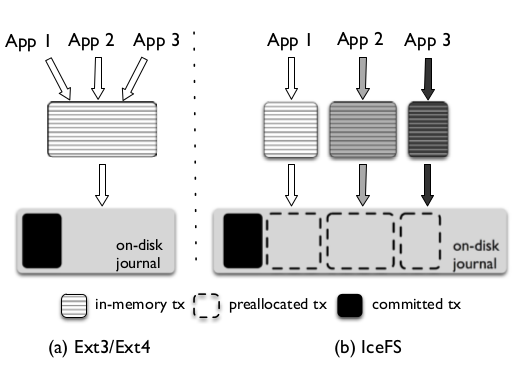
\includegraphics[scale=0.3]{./figures/fig7.png}
            \end{figure}
        \end{column}
    \end{columns}
\end{frame}

\section{Benefits of IceFS}
\begin{frame}{Localized Reactions to Failures}
    \bi
\item Fault detection:
    \bi
\item IceFS modifies existing detection techniques to make them cube-aware.
\item Instruments fault-handling and crash-triggering functions to include the
    ID of responsible cube.
    \ei
\item Localized Read-Only:
    \bi
\item Individually aborts transactions for a single cube.
\item Faulty cube alone is made read-only.
    \ei
\item Localized Crashes:
    \bn
\item Fails the crash-triggering thread.
\item Prevent new threads.
\item Evacuates running threads.
\item Clean up the cube.
    \en
    \ei
\end{frame}

\begin{frame}{Localized Recovery} 
    \bi
\item Offline Checking: 
    \bi
\item Supports partial checking of a file system by examining
    only faulty cubes.
\item ice-fsck identifies, checks, and repairs the faulty cube alone.
    \ei
\item Online Checking:
    \bi
\item Offline checking implies data will be unavailable, which is not acceptable
    for many applications.
\item IceFS enables on-line checking of faulty cubes alone.
\item Online ice-fsck is a user-space program that takes the ID of the faulty
    cube.
    \ei
    \ei
\end{frame}

\begin{frame}{Specialized Journaling}
    \bi
\item Since there are no dependencies across cubes, different consistency modes
    for cubes.
\item Five consistency modes:
    \bn
\item no fsync
\item no journal
\item writeback journal
\item ordered journal
\item data journal
    \en
    \ei
\end{frame}

\section{Implementation \& Evaluation}
\begin{frame}{Implementation}
    \bi
\item Ext3/JBD in Linux 3.5 was modified for data structures and journaling
    isolation.
\item VFS for directory indirection.
\item e2fsprogs 1.42.8 for file system creation and checking.
    \ei
\end{frame}

\begin{frame}{Overall Performance}
    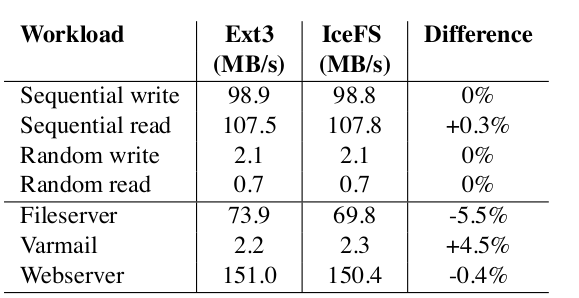
\includegraphics[scale=0.6]{./figures/table3.png}
\end{frame}

\begin{frame}{Evaluation}
    \begin{columns}[T]
        \begin{column}{0.4\textwidth}
            \begin{figure}
                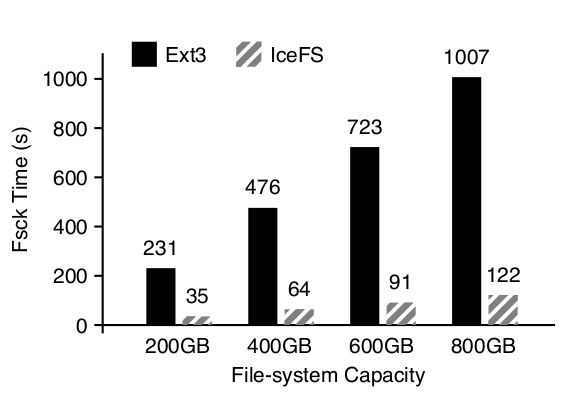
\includegraphics[scale=0.3]{./figures/fig8.png}
                \caption{Performance of IceFS Offline Fsck.}
            \end{figure}
        \end{column}
        \begin{column}{0.4\textwidth}
            \begin{figure}
                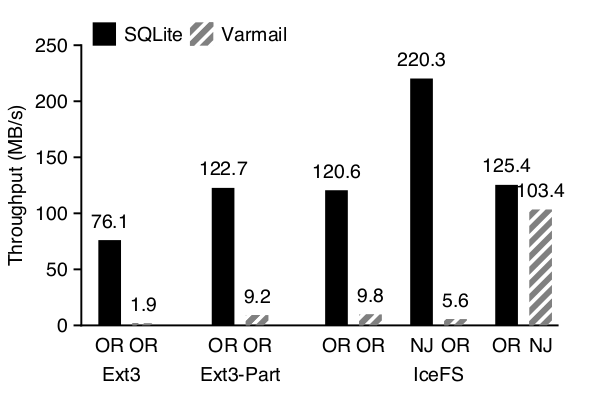
\includegraphics[scale=0.3]{./figures/fig9.png}
                \caption{IceFS under different journaling modes.}
            \end{figure}
        \end{column}
    \end{columns}
\end{frame}

\section{Limitations}
\begin{frame}{Limitations}
    \begin{columns}[T]
        \hspace{-4cm}\begin{column}{0.3\textwidth}
        \bi
    \item IceFS uses separate journal commit thread for every cube.
        \ei
    \end{column}
    \pause
    \hspace{-2cm}\begin{column}{0.3\textwidth}
        \begin{figure}
            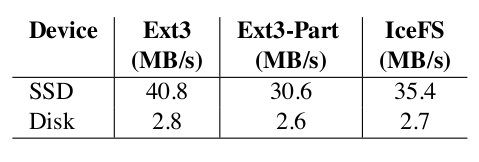
\includegraphics[scale=0.43]{./figures/table4.png}
        \end{figure}
    \end{column}
    \end{columns}
    \pause
    \bi
\item Cache flush time accounts for more in SSD, while seek times dominate in
    hard drives.
    \ei
\end{frame}

\begin{frame}{References}
\begin{thebibliography}{9}
    \bibitem{liu14}Lu, L., Zhang, Y., Do, T., Al-Kiswany, S., Arpaci-Dusseau, A.
    C., \& Arpaci-Dusseau, R. H. (2014). Physical disentanglement in a
    container-based file system. In 11th USENIX Symposium on Operating Systems
    Design and Implementation (OSDI 14) (pp. 81-96).
\end{thebibliography}
\end{frame}



\end{document}
